\chapter{Экспериментальные исследования алгоритма классификации сигналов фМРТ}

\section{Описание исходных данных}

S
 задач

 примеров

 испытуемых

 временные отсчёты

\begin{figure}%
	\begin{center}
		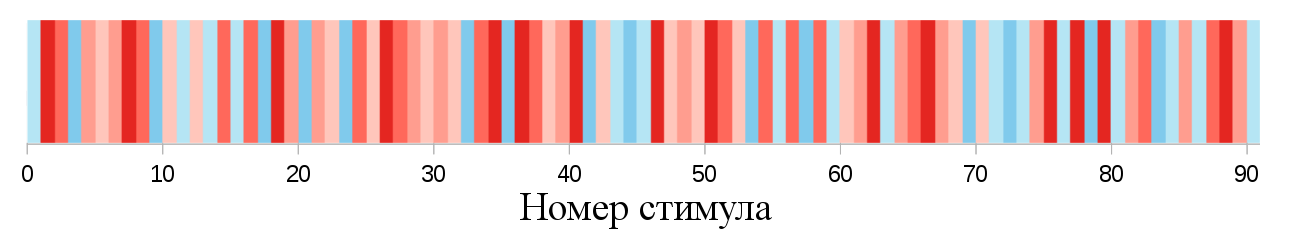
\includegraphics[width=.8\columnwidth]{./img/exp_design.png}%
	\end{center}
	\caption{Дизайн эксперимента.\\
		 Оттенки красного обозначают стимулы типа \textbf{V}, синего --- стимулы типа \textbf{S} }%
	\label{pic:exp_dis}%
\end{figure}

Воксели и Мозги во времени

На рисунке \ref{pic:local_100c} представлен результат работы набора команд представленного в приложении \ref{code:plt}
\begin{figure}%
	\begin{center}
		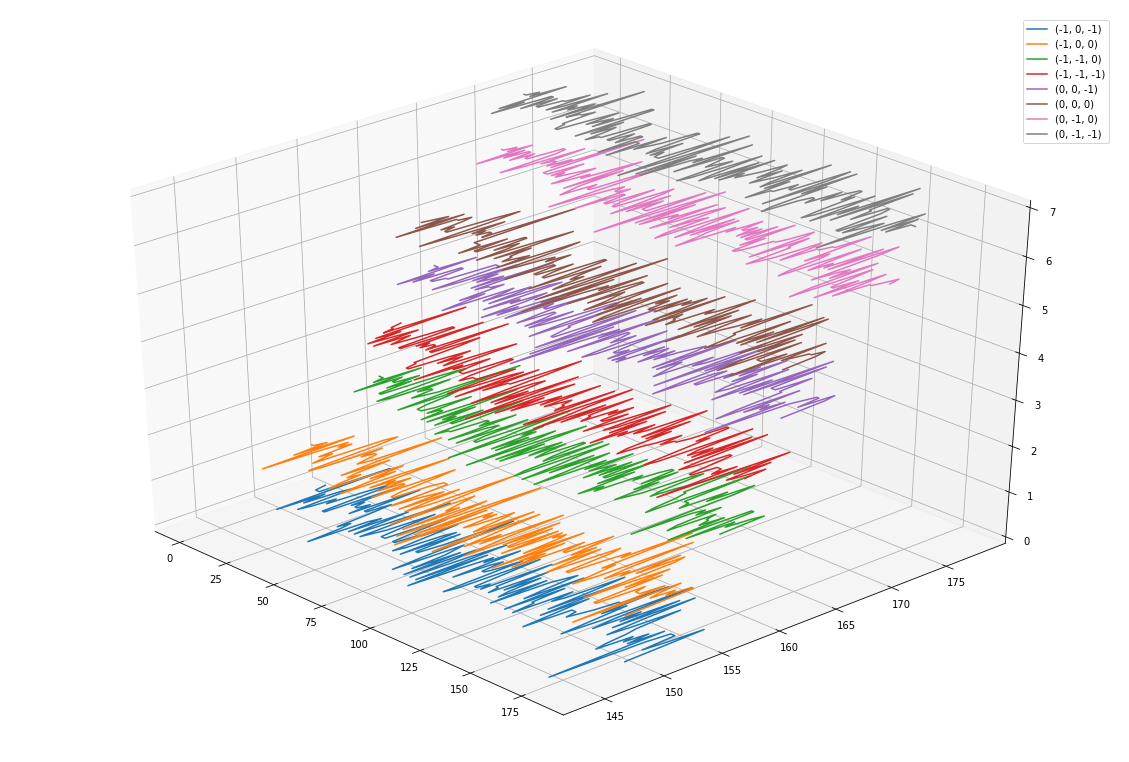
\includegraphics[width=.4\columnwidth]{./img/local_100c.png}%
	\end{center}
	\caption{Пример активности локальной окрестности вокселя в течение $\approx47$ сек}%
	\label{pic:local_100c}%
\end{figure}

\begin{figure}%
	\begin{center}
		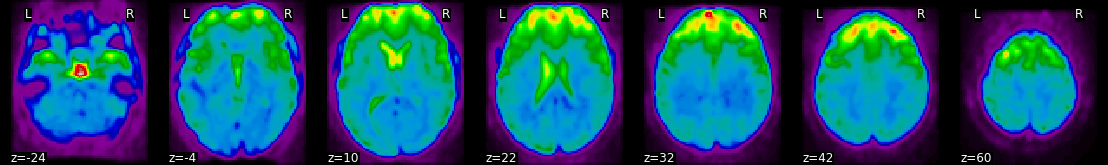
\includegraphics[width=.9\columnwidth]{./img/slices.png}%
	\end{center}
	\caption{Разрезы мозга по $z$-координате}%
	\label{pic:slices}%
\end{figure}

\section{Составление плана экспериментальных исследований разработанного алгоритма}

Что хотим

Параметры точности

Вопросы, ответы на которые хотим получить

При каком числе вокселей лучше точность

\section{Исследование точности классификации при различных	способах оценки межиндивидуальных корреляций}

\section{Исследование показателей точности классификации, выявление наименее и наиболее разделимых когнитивных состояний и соответствующих зон головного мозга}

Графики, таблицы

ROC, AUC

4000

\begin{table}%
	\caption{Результаты многоклассовой классификации}\label{tbl:mul_res}%
	\centering
	\begin{tabu}{|X[1.1]|X|X|X|X|}
		\hline
		Признак               & Точность & Полнота & $f1$-мера & Количество \\ \hline
		S1                     & $0.77$     & $0.69$    & $0.73$      &$90$         \\ \hline
		S2                    & $0.69$     & $0.80$    & $0.74$      &$87$         \\ \hline
		V1                     & $0.72$     &$0.67$    &$0.70$      &$85$         \\ \hline
		V2                    &$0.67$     &$0.63$    &$0.65$      &$82$         \\ \hline
		V3                     &$0.73$     &$0.65$    &$0.69$      &$84$         \\ \hline
		V4                     &$0.59$     &$0.68$    &$0.63$      &$81$         \\ \hline
		Среднее / Всё &$0.69$     &$0.69$    &$0.69$      &$509$        \\ \hline
	\end{tabu}
\end{table}

\begin{table}%
	\caption{Результаты многоклассовой для метода выделения t-статистики классификации}\label{tbl:mul_tstat_res}%
	\centering
	\begin{tabu}{|X[1.1]|X|X|X|X|}
		\hline
		Признак       & Точность & Полнота & $f1$-мера & Количество \\ \hline
		S1            &$ 0.65$     &$ 0.70$    &$ 0.67$      &$ 88$         \\ \hline
		S2            &$ 0.61$     &$ 0.68$    &$ 0.64$      &$ 80$         \\ \hline
		V1            &$ 0.70$     &$ 0.66$    &$ 0.68$      &$ 88$         \\ \hline
		V2            &$ 0.55$     &$ 0.65$    &$ 0.60$      &$ 71$         \\ \hline
		V3            &$ 0.78$     &$ 0.70$    &$ 0.74$      &$ 89$         \\ \hline
		V4            &$ 0.72$     &$ 0.62$    &$ 0.67$      &$ 92$         \\ \hline
		Среднее / Всё &$ 0.68$     &$ 0.67$    &$ 0.67$      &$ 508$        \\ \hline
	\end{tabu}
\end{table}


Бинарные признаки --- объединение всех одинакового типа (S*, V*)в$ 2$ группы

\begin{table}%
	\caption{Результаты классификации для бинарных признаков}\label{tbl:bin_res}%
	\centering
\begin{tabu}{|X[1.1]|X|X|X|X|}
	\hline
	Признак               & Точность & Полнота   & $f1$-мера & Количество \\ \hline
	S*                    & $0.95 $  & $ 0.82$   & $0.88$    & $ 170$     \\ \hline
	V*                    & $ 0.91 $ & $  0.98 $ & $ 0.94 $  & $  339$    \\ \hline
	Среднее / Всё & $0.92$   & $0.92 $   & $0.92$    & $509$      \\ \hline
\end{tabu}
\end{table}
Полученный результат находится на уровне state-of-the-art классификатора для разреженных данных по версии \cite{zhang2013some}.

\subsubsection*{Валидация}
В качестве подтверждения значимости шага сегментации при помощи ISC воспользуемся выбором случайных вокселей и их окрестностей в качестве признаков для классификатора:

\begin{table}%
	\caption{Результаты классификации для бинарных признаков при случайном выборе значимых вокселей}\label{tbl:rnd_res}%
	\centering
	\begin{tabu}{|X[1.1]|X|X|X|X|}
		\hline
		Признак       & Точность & Полнота & $f1$-мера & Количество \\ \hline
		S*            & $0.78$   & $0.83$  & $0.80$    & $168$      \\ \hline
		V*            & $0.91$   & $0.89$  & $0.90$    & $341$      \\ \hline
		Среднее / Всё & $0.87$   & $0.87$  & $0.87$    & $509$      \\ \hline
	\end{tabu}
\end{table}


\begin{table}%
	\caption{Результаты классификации для бинарных признаков при выборе значимых вокселей  c помощью метода t-статистики}\label{tbl:ttest_res}%
	\centering
	\begin{tabu}{|X[1.1]|X|X|X|X|}
		\hline
		Признак       & Точность & Полнота & $f1$-мера & Количество \\ \hline
		S*            & $0.95$   & $0.85$  & $0.90$    & $168$      \\ \hline
		V*            & $0.93$   & $0.98$  & $0.95$    & $340$      \\ \hline
		Среднее / Всё & $0.94$   & $0.94$  & $0.93$    & $508$      \\ \hline
	\end{tabu}
\end{table}

\begin{table}%
	\caption{Результаты классификации для бинарных признаков при выборе значимых вокселей  c помощью метода GLM}\label{tbl:glm_res}%
	\centering
	\begin{tabu}{|X|X|X|X|X|}
		\hline
		Признак       & Точность & Полнота & $f1$-мера & Количество \\ \hline
		S*            &$ 0.85$     &$ 0.88$    &$ 0.87$      &$ 146$        \\ \hline
		V*            &$ 0.95$     &$ 0.94$    &$ 0.94$      &$ 362$        \\ \hline
		Среднее / Всё &$ 0.92$     &$ 0.92$    &$ 0.92$      &$ 508$        \\ \hline
	\end{tabu}
\end{table}